This section contains more results of the experiment from \cref{sec:TraceComparisonExperiment}. The results for loss functions of order 4 and 6 for the network of width 128 are depicted in \cref{fig:MNISTTraceComparison1} and \cref{fig:MNISTTraceComparison2}. The results for loss functions of order 2, 4 and 6 for the network of width 784 are depicted in \cref{fig:MNISTTraceComparison3}, \cref{fig:MNISTTraceComparison4} and \cref{fig:MNISTTraceComparison5}. The Cross-entropy loss doesn't vary with order but is still depicted for reference in every plot.

\begin{figure}
	\centering
	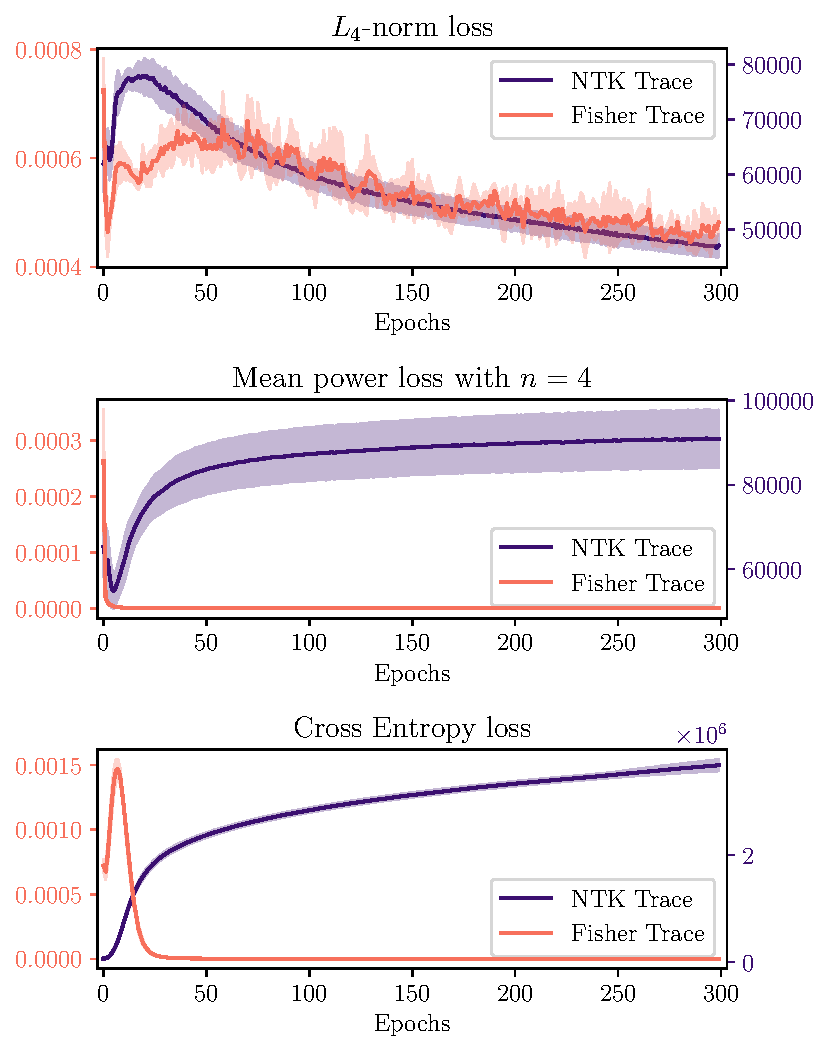
\includegraphics[width=\textwidth]{text/results/FisherNTKComparisonPlots/Triple_comparison_losses4_128.pdf}
	\caption{Trace of NTK and Fisher information during 300 epochs of training on the MNIST dataset using the Adam optimizer. The network consisted of 2 hidden layers with a \emph{width of 128 neurons} that were equipped with the ReLU activation function. The loss functions used for optimization are denoted in each subplot. The solid line represents the mean value of 5 experiments, the translucent area represents one standard deviation from the mean value.}
	\label{fig:MNISTTraceComparison1}
\end{figure}
\begin{figure}
	\centering
	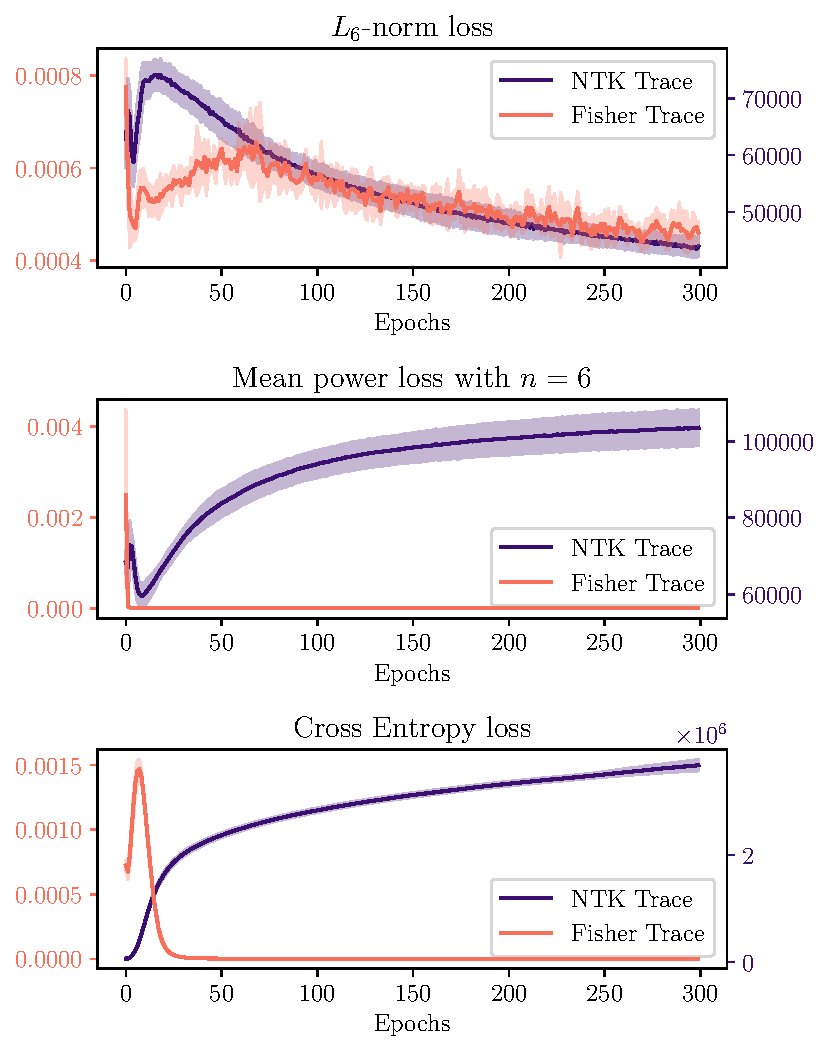
\includegraphics[width=\textwidth]{text/results/FisherNTKComparisonPlots/Triple_comparison_losses6_128.pdf}
	\caption{Trace of NTK and Fisher information during 300 epochs of training on the MNIST dataset using the Adam optimizer. The network consisted of 2 hidden layers with a \emph{width of 128 neurons} that were equipped with the ReLU activation function. The loss functions used for optimization are denoted in each subplot. The solid line represents the mean value of 5 experiments, the translucent area represents one standard deviation from the mean value.}
	\label{fig:MNISTTraceComparison2}
\end{figure}
\begin{figure}
	\centering
	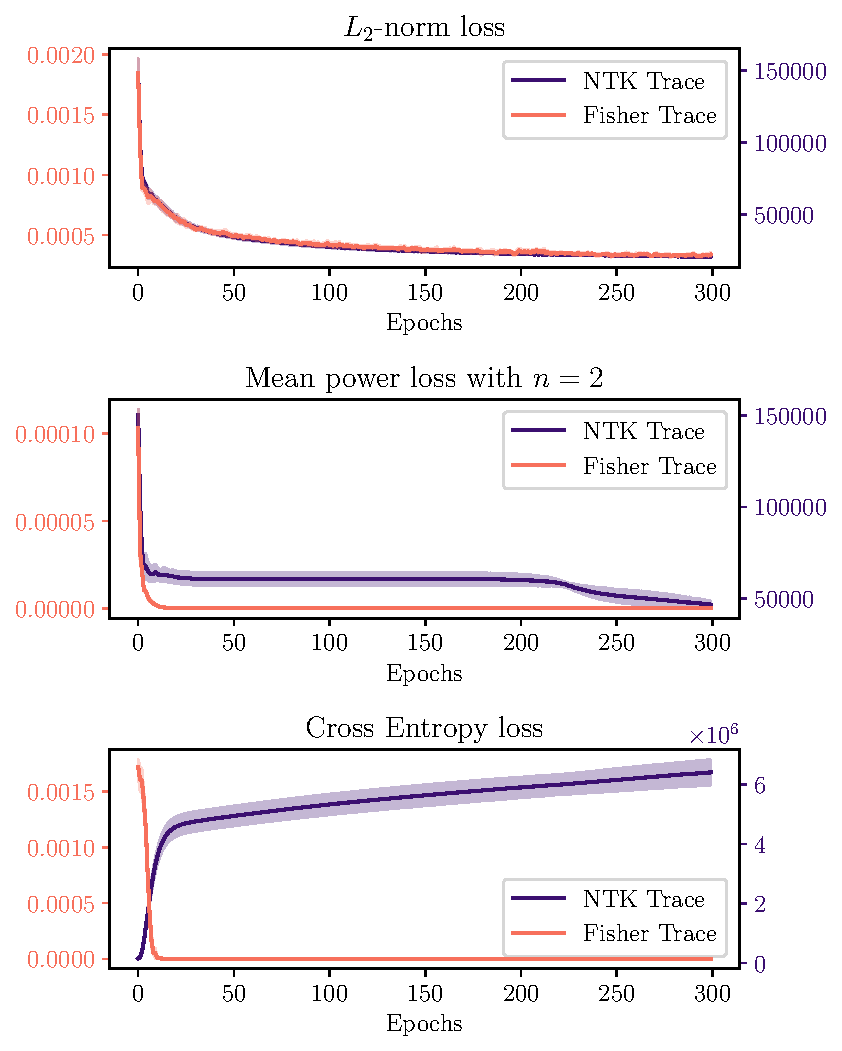
\includegraphics[width=\textwidth]{text/results/FisherNTKComparisonPlots/Triple_comparison_losses2_784.pdf}
	\caption{Trace of NTK and Fisher information during 300 epochs of training on the MNIST dataset using the Adam optimizer. The network consisted of 2 hidden layers with a \emph{width of 784 neurons} that were equipped with the ReLU activation function. The loss functions used for optimization are denoted in each subplot. The solid line represents the mean value of 5 experiments, the translucent area represents one standard deviation from the mean value.}
	\label{fig:MNISTTraceComparison3}
\end{figure}
\begin{figure}
	\centering
	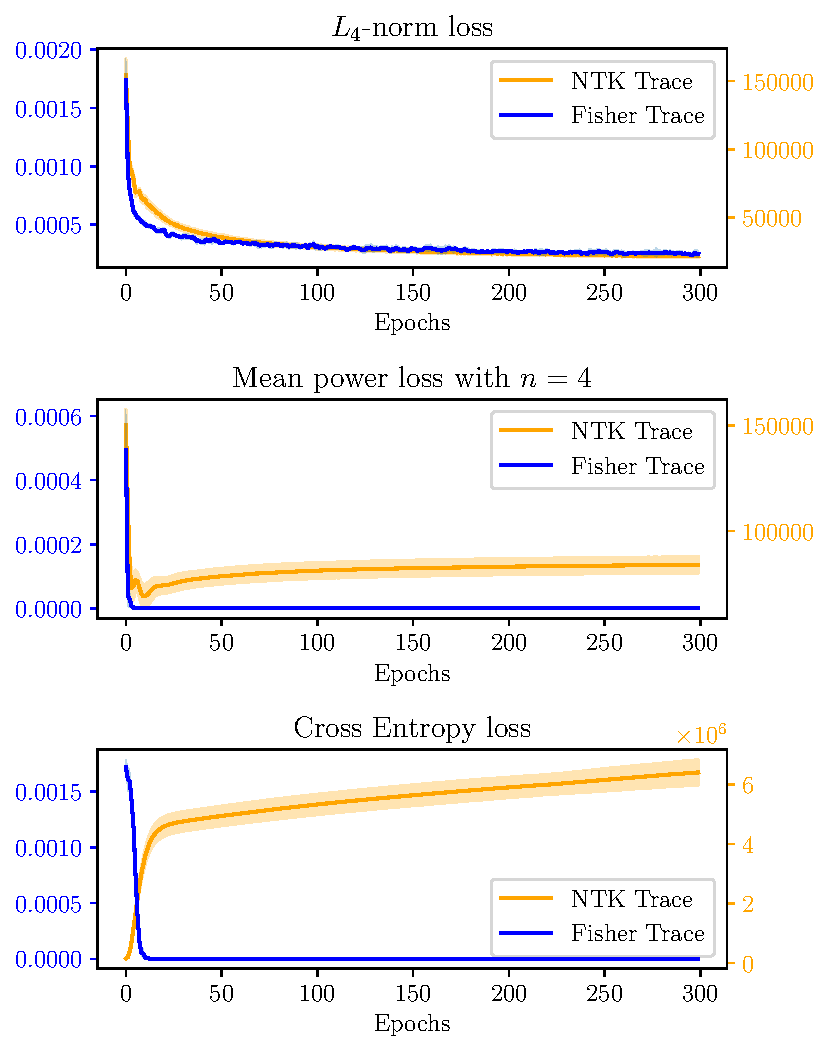
\includegraphics[width=\textwidth]{text/results/FisherNTKComparisonPlots/Triple_comparison_losses4_784.pdf}
	\caption{Trace of NTK and Fisher information during 300 epochs of training on the MNIST dataset using the Adam optimizer. The network consisted of 2 hidden layers with a \emph{width of 784 neurons} that were equipped with the ReLU activation function. The loss functions used for optimization are denoted in each subplot. The solid line represents the mean value of 5 experiments, the translucent area represents one standard deviation from the mean value.}
	\label{fig:MNISTTraceComparison4}
\end{figure}
\begin{figure}
	\centering
	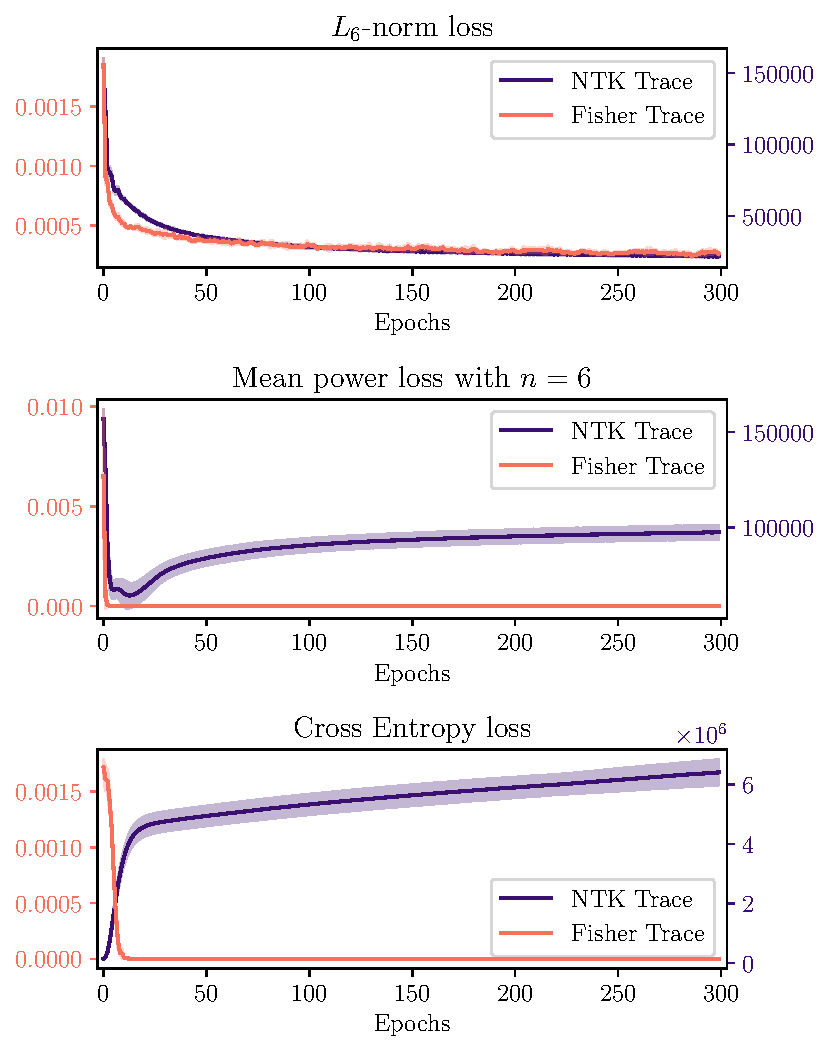
\includegraphics[width=\textwidth]{text/results/FisherNTKComparisonPlots/Triple_comparison_losses6_784.pdf}
	\caption{Trace of NTK and Fisher information during 300 epochs of training on the MNIST dataset using the Adam optimizer. The network consisted of 2 hidden layers with a \emph{width of 784 neurons} that were equipped with the ReLU activation function. The loss functions used for optimization are denoted in each subplot. The solid line represents the mean value of 5 experiments, the translucent area represents one standard deviation from the mean value.}
	\label{fig:MNISTTraceComparison5}
\end{figure}